\documentclass[11pt,a4paper]{article}
\usepackage[T1]{fontenc}
\usepackage[utf8]{inputenc}
\usepackage{lmodern,microtype}
\usepackage[margin=24mm,headheight=15pt]{geometry}
\usepackage{amsmath,amssymb,amsthm,mathtools}
\usepackage{booktabs,longtable,array,tabularx}
\usepackage{enumitem,xurl}
\usepackage{tocloft}
\setlength{\cftbeforesecskip}{3pt}
\usepackage{tikz}
\usepackage[hidelinks]{hyperref}
\usepackage{fancyhdr}
\pagestyle{fancy}\fancyhf{}
\fancyhead[L]{\small Projective port atlases}
\fancyhead[R]{\small ProveIt research continuation}
\fancyfoot[C]{\thepage}
\setlength{\parskip}{4pt}\setlength{\parindent}{0pt}
\setlength{\emergencystretch}{3em}
\setlist{nosep,leftmargin=*,topsep=4pt}
\newtheorem{theorem}{Theorem}[section]
\newtheorem{lemma}[theorem]{Lemma}
\newtheorem{proposition}[theorem]{Proposition}
\newtheorem{corollary}[theorem]{Corollary}
\theoremstyle{definition}
\newtheorem{definition}[theorem]{Definition}
\newtheorem{example}[theorem]{Example}
\theoremstyle{remark}
\newtheorem{remark}[theorem]{Remark}
\newcommand{\R}{\mathbb R}\newcommand{\Q}{\mathbb Q}\newcommand{\Z}{\mathbb Z}
\newcommand{\supp}{\operatorname{supp}}\newcommand{\rank}{\operatorname{rank}}
\newcommand{\cone}{\operatorname{cone}}\newcommand{\conv}{\operatorname{conv}}
\newcommand{\spanlin}{\operatorname{span}}\newcommand{\poly}{\operatorname{poly}}
\newcommand{\one}{\mathbf1}\newcommand{\code}[1]{\texttt{\detokenize{#1}}}
\newcommand{\pos}{\textsf{POSITIVE}}\newcommand{\nonpos}{\textsf{NO\_POSITIVE}}
\newcommand{\pin}{\texttt{74de08949619863b002b5fcf01813a2faddde212}}
\newcommand{\NormalBase}{402.745}
\newcommand{\NormalSplit}{19.751}
\newcommand{\NormalRatio}{20.39}
\newcommand{\ModeRatio}{166.35}

\hypersetup{pdftitle={Projective Port Atlases for Normal-Surface Discovery},pdfauthor={Research continuation for Vladimir Reshetnikov; developed with ChatGPT},pdfsubject={Higher-rank interfaces, exact compatible cone search, normal-surface witnesses}}
\title{\textbf{Projective Port Atlases\\for Normal-Surface Discovery}\\[7pt]
\large Objective-independent higher-rank interfaces,\\source-exact compilation, and connected witnesses}
\author{Research continuation for Vladimir Reshetnikov's ProveIt project\\
\small Mathematical development and implementation assisted by ChatGPT}
\date{12 October 2026}
\begin{document}
\maketitle
\begin{abstract}
We develop an exact discovery kernel for nonnegative matching equations with local coordinate incompatibilities. Several independently complicated pieces are required to share one $d$-coordinate port. Instead of enumerating the Cartesian product of their compatibility choices, we normalize the common port and construct a finite arrangement determined only by local admissible rays. After separating positive zero-port directions, every remaining objective and coordinate-zero restriction attains its nonzero-port optimum at a vertex of this same arrangement. With two ports, the atlas consists only of the distinct normalized local ray images: intersections of objective lines are unnecessary.

The direct exact implementation has bit complexity $\poly(\Lambda)(R+d+1)^{d^2-d+1}$ after local ray enumeration, where $R$ is the total number of local admissible rays and $\Lambda$ measures the encoded input. If local blocks have at most $k$ variables, a complete support enumerator gives $\poly(\Lambda)\exp(O(d^2(k+\log(m+d+2))))$. Thus logarithmic block size and port dimension give a cubic-logarithm quasi-polynomial bound for this complete discovery problem. An alternative enumerator allows large blocks of bounded algebraic nullity. The synchronization hypothesis is essential; arbitrary width-two chains already encode exact cover.

Two source compilers preserve all matching equations and conflicts. We also show why primitive assembled vectors cannot automatically be called source rays, and give a polynomial-bit support descent that produces primitive extreme witnesses. For authenticated standard normal coordinates, these witnesses are connected. The package includes 46 unit tests, 960 random-model queries, 104 queries on a repository normal fixture, independent checks, and 64 nonextreme-to-extreme recovery examples. Seven paired full source-query trials improve from \NormalBase\,ms to \NormalSplit\,ms against the delivered unsplit enumerator. These are local discovery results, not a general quasi-polynomial unknot recognizer or a native production benchmark.
\end{abstract}
\vspace{5pt}
\noindent\textbf{Reference revision.} \pin.\quad
\textbf{Delivery.} Editable proofs, exact standard-library Python, independent checks, raw measurements, and additive integration notes.
\clearpage
\begingroup\footnotesize\setlength{\parskip}{0pt}\tableofcontents\endgroup
\clearpage
\section{Research position and the improvement pursued}
\label{sec:position}

\subsection{Discovery rather than another supplied-surface observer}
The inspected ProveIt material distinguishes a complete exact recognizer from its many compressed geometric and algebraic operators. Its README explicitly does not assert a general quasi-polynomial bound. The recent catalogue contains work on raw normal cuts, normal-coordinate sectors, source-certified interfaces, cancellation, and hierarchy bookkeeping. Report 96 addresses a different but equally necessary task: discovering a positive-objective admissible vector without multiplying all local compatibility searches \cite{repo,scalar}.

This article continues that discovery direction. Its input is not a supplied normal surface; it is a finite source system whose useful surface is to be found. The output is a positive matching vector, or a complete negative answer to the specified algebraic query. For a positive answer, we can additionally produce and independently check an extreme source ray. The normal-surface interpretation is invoked only after the source equations have been authenticated.

The mathematical opportunity is that many independent local choices may meet the \emph{same} small interface. A direct implementation would select a compatibility mode in each piece and solve every global combination. We instead choose a finite set of interface values at which the local pieces can be optimized independently. The central issue is completeness: the set must not omit boundary strata, introduce incompatible mixtures, or depend on a particular Euler objective.

\subsection{Relation to the announced target}
Lackenby's 2021 slides state an $n^{O(\log n)}$ unknot-recognition bound. The July 2026 preprint develops a hierarchy algorithm, while its Section 9 deliberately separates iteration counting from the insufficiently specified cost of several operations. Its displayed iteration estimate is $L(g+1)^L$, in terms of hierarchy length and pattern complexity \cite{slides,lack2026}. A faster local search is therefore useful without being an end-to-end complexity theorem.

Our most general implemented bound has logarithm
\begin{equation}
 O\bigl(d^2(k+\log(m+d+2))\bigr)+O(\log\Lambda),
 \label{eq:headline-log}
\end{equation}
under the definitions below. Logarithmic $d$ and $k$, with polynomially bounded source size, give $2^{O((\log n)^3)}$. Obtaining the stronger $n^{O(\log n)}$ target through this kernel requires the expression in \eqref{eq:headline-log} to be $O((\log n)^2)$, together with compatible bounds for all other operations. These exponents are not interchangeable.

\subsection{What is new in the present development}
We do not claim novelty for normal matching cones, extreme-ray support tests, linear-programming bases, polyhedral arrangements, or parametric linear programming. These are established tools; normal-surface complexity and branching algorithms are discussed in \cite{bo,bps}, and parametric LP in \cite{parametric}. Nor do we claim an exhaustive literature-priority search.

The proposed additions are a \emph{single objective-independent atlas} for a synchronized family of locally incompatible cones; its particularly small two-port form; uniform reuse under all coordinate-zero restrictions; a higher-dimensional construction that handles lower-dimensional feasible domains explicitly; and a source-safe recovery contract that does not extend the scalar no-new-rays assertion without proof. The implementation and the measured source-query workload follow those exact theorems.

Report 96 summarizes arbitrary signed scalar subtrees by a few one-dimensional continuation data. Our hypothesis is different: higher-dimensional pieces share one master port, rather than recursively transporting distinct higher-dimensional ports along a tree. Neither result subsumes the other. In particular, this article does not claim to solve the general two-coordinate continuation problem left open by that report.

\subsection{Scope of the repository audit}
The reference revision is \pin. The source review was targeted: the main README, the synthesis introduction, the report catalogue through report 105, report 96's article entry point and README, and its complete fixture module were read through the GitHub connector. Some initial reads used the moving main branch; the returned blob identifiers are recorded in \code{SOURCE_AUDIT.md} rather than being silently treated as a verified full checkout.

Four ZIP archives were visible in \code{docs/incoming}: exceptional rows, matroidal dual forests, nonlinear activation forests, and ordered interface kernels. Their directory records were inspected, but the available binary-fetch routes did not provide their contents. We consequently make no claim of exhaustive overlap review of those deliveries. No upstream default, incoming archive, or numbered report was modified. The current package is an additive proposed continuation.

\section{The synchronized conic problem}
\label{sec:model}

\begin{definition}[Locally incompatible matching block]
For $1\le i\le m$, let
\[
 K_i=\{x_i\in\R^{n_i}_{\ge0}:A_i x_i=0\}
\]
with $A_i$ rational. A set $\mathcal F_i$ of unordered pairs of distinct coordinate indices specifies the admissible set
\[
 K_i^{\rm adm}=\{x_i\in K_i:x_{ia}x_{ib}=0\text{ for every }\{a,b\}\in\mathcal F_i\}.
\]
A rational map $P_i:\R^{n_i}\to\R^d$ is a nonnegative port map when $P_i x_i\ge0$ on $K_i$. The implementation uses the sufficient, directly checked hypothesis that every entry of $P_i$ is nonnegative.
\end{definition}

All cones are pointed because they lie in a nonnegative orthant. The feasible synchronized family is
\begin{equation}
 \mathcal X=\{(x_1,\ldots,x_m,y):x_i\in K_i^{\rm adm},\quad P_i x_i=y\ \ (1\le i\le m)\}.
 \label{eq:model}
\end{equation}
There are no additional, unrecorded cross-block conflicts. Given rational objectives $c_i,c_0$, and optional sets $Z_i$ of coordinates forced to zero, the query is whether
\begin{equation}
 \Phi(x,y)=c_0^Ty+\sum_{i=1}^m c_i^Tx_i>0
 \label{eq:objective}
\end{equation}
for some feasible tuple satisfying the zero restrictions. The zero tuple is always allowed but never answers the strict query positively.

Write $\mathcal R_i$ for the admissible extreme rays of the \emph{full} cone $K_i$, using primitive integer generators after clearing denominators. Set $R_i=|\mathcal R_i|$ and $R=\sum_iR_i$. A subset of rays is compatible when the union of their coordinate supports contains no forbidden pair. The number of local variables is $k=\max_i n_i$. The symbol $\Lambda$ denotes the full binary input length, including matrices, conflicts, dimensions and query data. Polynomial factors below may include ordinary coordinate-vector operations; they do not suppress an exponential dependence on $k$ or $d$.

\begin{lemma}[Support-respecting generation]
\label{lem:decomp}
Every admissible $x\in K_i$ is a nonnegative combination of mutually compatible rays in $\mathcal R_i$, each supported inside $\supp(x)$. The assertion remains true after arbitrary coordinate-zero restrictions.
\end{lemma}
\begin{proof}
For nonzero $x$, intersect $K_i$ with $\one^T x=1$. This is a compact rational polytope; its vertices correspond to extreme rays of $K_i$. Thus $x$ is a nonnegative combination of such rays. In a nonnegative sum, a coordinate that is zero in the sum is zero in every summand with a positive coefficient. Each participating ray is therefore supported inside $\supp(x)$. An admissible support contains no forbidden pair, so all participating rays are admissible and mutually compatible. The same argument preserves every forced zero.
\end{proof}

A useful consequence is that compatibility sectors need not be explicitly listed. One may enumerate all full-cone rays, discard inadmissible ones, and later test support unions. A face obtained by setting coordinates to zero has no new extreme rays: its rays are precisely the surviving full-cone rays. This fact is the basis of reusable anchor queries.

\subsection{Separating zero-port directions}
For a ray $r\in\mathcal R_i$, let
\[
 h_r=\one^TP_i r.
\]
Nonnegativity implies $h_r=0$ exactly when $P_i r=0$.

\begin{lemma}[Zero-port alternative]
\label{lem:zero}
If an unexcluded ray $r\in\mathcal R_i$ satisfies $h_r=0$ and $c_i^Tr>0$, then the synchronized query is positive. Otherwise, every zero-port feasible tuple has nonpositive objective, and any feasible nonzero-port tuple can be replaced, without decreasing its objective or changing its port, by one using only positive-port rays in each block.
\end{lemma}
\begin{proof}
A positive zero-port ray can be placed in its block with all other blocks zero. Conversely, decompose each local vector as in Lemma~\ref{lem:decomp}. When the total port is zero, nonnegative ray images force every participating image to be zero. By hypothesis every corresponding objective contribution is nonpositive. For a nonzero port, simply delete all zero-port ray summands. Each deletion preserves matching, admissibility, forced zeros and the port, and does not lower the objective.
\end{proof}

For the rest of the atlas construction, zero-port rays are omitted and the common port is normalized to
\[
 \Delta^{d-1}=\{y\in\R^d_{\ge0}:\one^Ty=1\}.
\]
Define the normalized source vector, port point and reward of a positive-port ray by
\begin{equation}
 v_r=r/h_r,\qquad p_r=P_i r/h_r,\qquad a_r=c_i^Tv_r.
 \label{eq:normalize}
\end{equation}
The ray's source vector and its port point must not be confused. Distinct source rays can have the same port point, different compatibility relations, and different rewards.

\section{Compatible simplices and the two-port theorem}
\label{sec:two}

\begin{lemma}[At most $d$ compatible rays at a fixed port]
\label{lem:simplex}
Suppose the positive zero-port alternative does not occur. If a block is feasible at $y\in\Delta^{d-1}$, its maximum objective at that port is attained by a convex combination of at most $d$ normalized rays. Their port points are affinely independent and their source supports are mutually compatible.
\end{lemma}
\begin{proof}
There are finitely many compatible subsets of rays. For any one such subset, the admissible coefficient vectors at port $y$ form
\[
 \{\alpha\ge0:\sum_r\alpha_rp_r=y\}.
\]
Applying $\one^T$ shows $\sum_r\alpha_r=1$, so this set is compact. The objective is $\sum_r\alpha_ra_r$. At an extreme point of the coefficient polytope, the columns $p_r$ with positive coefficients are linearly independent: otherwise a nonzero dependence permits small perturbations of both signs while keeping all positive coefficients nonnegative. There are at most $d$ such columns. Since every $p_r$ has coordinate sum one, linear independence of these columns is equivalent to affine independence of the points. Maximize over the finitely many compatible subsets and use Lemma~\ref{lem:zero} to discard nonpositive zero-port contributions.
\end{proof}

For a compatible independent set $S$, write $D_S=\conv\{p_r:r\in S\}$. At each $y\in D_S$ there is a unique barycentric expression in these points, and hence an affine reward $\ell_{i,S}(y)$. It is a function on the affine span of $D_S$; no arbitrary extension outside that span is needed. A block's optimal value is the maximum of these affine rewards over the simplexes containing $y$. The domain can be disconnected or lower-dimensional, and the maximum need not be globally concave.

\begin{theorem}[Two-port ray-image atlas]
\label{thm:two}
Let $d=2$. After checking positive zero-port rays, the strict query is decided by evaluating only the distinct normalized port points $p_r$ from all blocks. Equivalently, put
\[
 \mathcal T=\left\{\frac{(P_i r)_2}{\one^TP_i r}:r\in\mathcal R_i,\ h_r>0\right\},\qquad U=|\mathcal T|\le R.
\]
For each $t\in\mathcal T$, independently maximize the local reward among admissible single rays at slope $t$ and compatible pairs bracketing $t$. If all blocks are feasible, add their rewards and $c_0^T(1-t,t)$. The maximum over these tests equals the global normalized optimum. The same set $\mathcal T$ works for every objective and every coordinate-zero restriction.
\end{theorem}
\begin{proof}
By Lemma~\ref{lem:simplex}, local candidates are points or closed intervals with affine rewards, whose endpoints lie in $\mathcal T$. Sort the distinct slopes. Take any normalized feasible point $t$ with its maximizing local candidates. If $t\in\mathcal T$, it is already tested. Otherwise $t$ lies strictly between two consecutive slopes $u<v$. Every chosen interval containing $t$ contains all of $[u,v]$: an interval endpoint cannot lie inside $(u,v)$ by definition of consecutiveness. The chosen total reward is affine on $[u,v]$, so it is at least its value at $t$ at one endpoint. All its local candidates are feasible at that endpoint. The independently reoptimized endpoint value is no smaller.

There is no feasible point strictly outside the smallest and largest slopes, because every feasible local port is a convex combination of local ray images. Consequently no extra endpoint is required unless it is itself a ray slope. Forced zeros delete rays and candidate intervals; using the original, possibly larger slope set still refines every remaining interval. The proof never used the objective values to construct $\mathcal T$.
\end{proof}

\begin{remark}[Why reward-line intersections are unnecessary]
On an open interval between consecutive domain endpoints, the available local affine pieces are fixed. Their pointwise maxima, and the sum of these maxima, are convex there. Maximizing such a function needs only the interval endpoints. The proof above is stronger than an appeal to global convexity: it remains valid when new pieces appear only at an endpoint or when the feasible set is disconnected. It is the endpoints of \emph{domains}, not crossings of reward lines, that matter.
\end{remark}

For normalized ray slopes $s<t$ with rewards $a_s,a_t$, the reward at $u\in[s,t]$ is
\[
 \frac{t-u}{t-s}a_s+\frac{u-s}{t-s}a_t.
\]
Pairs with equal slopes never improve on the better singleton. They need not be mixed, especially when their source supports are incompatible.

\begin{corollary}[Direct two-port cost]
\label{cor:two-cost}
After local rays are known, preparation and one query require at most
\[
 O\!\left(U\sum_{i=1}^m(R_i+R_i^2)\right)
\]
exact rational operations, apart from sorting, coordinate-support work and polynomial-size linear-algebra factors. Barycentric mixtures may be cached once and reused for arbitrarily many objectives and coordinate-zero faces.
\end{corollary}
\begin{proof}
There are at most $R_i$ singleton candidates and $\binom{R_i}{2}$ pair candidates in block $i$. At each of the $U$ slopes, test interval membership, compatibility and the affine reward. Caching their coefficients removes repeated interpolation from later queries. All tests use exact rational comparisons.
\end{proof}

\section{A finite atlas in every port dimension}
\label{sec:atlas}
The two-port theorem does not extend by keeping only ray images. In three ports, two feasible line segments can meet at a point that is a ray image of neither block. An arrangement of simplex boundary hyperplanes captures the missing points without introducing objective-dependent walls.

\subsection{The coordinate-frame construction}
Let $E=\{e_1,\ldots,e_d\}$ be the standard coordinate frame. In each block, combine its distinct positive-port points with $E$. For every linearly independent $(d-1)$-subset of this set, retain the hyperplane through its span. Let $\mathcal H$ be the union of these hyperplanes over all blocks, with duplicates removed. Hyperplanes are stored by primitive integer normal vectors, up to sign.

The frame ensures that $\mathcal H$ contains $y_j=0$ for every $j$. Define $\mathcal V$ to consist of all points of $\Delta^{d-1}$ obtained as a unique intersection of $\one^Ty=1$ and $d-1$ hyperplanes in $\mathcal H$. For $d=1$, define $\mathcal V=\{(1)\}$. Hyperplanes whose normals are dependent, inconsistent intersection systems, and intersections outside the nonnegative simplex are discarded by exact arithmetic.

\begin{lemma}[Every compatible simplex is an arrangement subcomplex]
\label{lem:frame}
Every $D_S$ is a union of closed cells of the hyperplane arrangement $\mathcal H$ inside $\Delta^{d-1}$. This includes simplexes of all dimensions, not just full-dimensional ones.
\end{lemma}
\begin{proof}
Suppose $S$ has $r\le d$ independent port columns $p_1,\ldots,p_r$. Complete these columns to a basis of $\R^d$ by choosing $d-r$ vectors from $E$; this is possible because $E$ spans the ambient space. Write the resulting basis as
\[
 B=(p_1,\ldots,p_r,e_{j_1},\ldots,e_{j_{d-r}}).
\]
In the corresponding basis coordinates, membership in $D_S$ means that the last $d-r$ coordinates vanish, the first $r$ are nonnegative, and the ambient normalization holds. When the last coordinates vanish, normalization makes the sum of the first $r$ coordinates equal one because each $p_i$ has coordinate sum one.

The vanishing hyperplane for each basis coordinate is spanned by the other $d-1$ basis vectors. All these vectors come from the same local point set together with $E$, so every such hyperplane belongs to $\mathcal H$. Thus the affine-span equations and all supporting facets of $D_S$ are arrangement hyperplanes. On a relatively open arrangement cell, all their signs are fixed. If one point of that cell lies in $D_S$, the whole cell does; its closure lies there as well because $D_S$ is closed. This proves the assertion.
\end{proof}

\begin{theorem}[Universal projective atlas]
\label{thm:atlas}
After the zero-port alternative is checked, the maximum of every normalized synchronized objective is attained at a point of $\mathcal V$, whenever a nonzero port is feasible. The set $\mathcal V$ depends only on the local cones, conflicts and port maps. It remains complete for every collection of coordinate-zero restrictions.
\end{theorem}
\begin{proof}
By the preceding lemmas, the normalized feasible set is a finite union of intersections of compatible local simplexes. These are compact. On each such intersection, the selected total reward is affine; hence a finite global maximum exists whenever the feasible set is nonempty.

Alternatively, start with any feasible tuple, remove nonpositive zero-port summands, and choose maximizing compatible simplex representations at its port $y$. Let $C$ be the relatively open arrangement cell containing $y$. By Lemma~\ref{lem:frame}, every chosen simplex contains $\overline C$. The chosen total reward is affine on this compact polytope, so one of its vertices $v$ has reward at least the reward at $y$. Reoptimizing the blocks at $v$ can only increase that value.

Every vertex of an arrangement cell in the $(d-1)$-dimensional affine space $\one^Ty=1$ is specified by $d-1$ independent active arrangement hyperplanes, including coordinate hyperplanes when necessary. Thus $v\in\mathcal V$. Lower-dimensional cells are covered by the same argument. Setting source coordinates to zero merely deletes rays and simplexes, and the original arrangement still refines each surviving simplex. No objective coefficient was used in constructing the arrangement.
\end{proof}

\subsection{The three-port intersection example}
\begin{example}[A required point absent from all ray images]
\label{ex:centroid}
Take two two-ray orthant blocks with no conflicts. Their integer port columns are
\[
 P_1=((2,0,0)^T,(0,1,1)^T),\qquad
 P_2=((0,2,0)^T,(1,0,1)^T).
\]
Their normalized domains are the medians joining $e_1$ to $(e_2+e_3)/2$ and $e_2$ to $(e_1+e_3)/2$. Their intersection is the singleton
\[
 y_*=(1/3,1/3,1/3).
\]
It is not a local ray image, but it is an arrangement vertex. For objective one on every source coordinate, the total normalized reward is one. An atlas restricted to ray images would falsely report no nonzero common port.
\end{example}

\begin{figure}[ht]
\centering
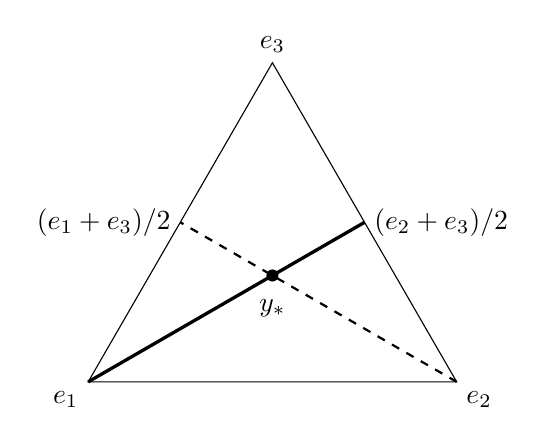
\begin{tikzpicture}[scale=.78]
\coordinate (A) at (0,0);\coordinate (B) at (6,0);\coordinate (C) at (3,5.196);
\coordinate (D) at (4.5,2.598);\coordinate (E) at (1.5,2.598);\coordinate (G) at (3,1.732);
\draw (A)--(B)--(C)--cycle;
\draw[very thick] (A)--(D);\draw[thick,dashed] (B)--(E);
\fill (G) circle (2.8pt);
\node[below left] at (A) {$e_1$};\node[below right] at (B) {$e_2$};\node[above] at (C) {$e_3$};
\node[right] at (D) {$(e_2+e_3)/2$};\node[left] at (E) {$(e_1+e_3)/2$};
\node[below,yshift=-5pt] at (G) {$y_*$};
\end{tikzpicture}
\caption{The two blocks are feasible on the solid and dashed medians, respectively. Their only common normalized port is a new intersection point. The figure concerns exact rational domains, not a geometric normal-surface embedding.}
\end{figure}

\section{Complete enumeration and binary complexity}
\label{sec:complexity}

\subsection{A deliberately simple complete local enumerator}
\begin{proposition}[Support characterization of rays]
\label{prop:support}
For a nonzero $x\in K_i$ with support $S$, its ray is extreme in $K_i$ exactly when
\[
 \dim\ker(A_i|_S)=1.
\]
Consequently, enumerating all nonempty coordinate supports, checking compatibility, testing one-dimensional nullity, and retaining the strictly positive kernel generators produces every admissible extreme ray exactly once.
\end{proposition}
\begin{proof}
If the support kernel has dimension greater than one, choose a vector in it not proportional to $x$. Sufficiently small perturbations of both signs remain positive on $S$ and zero elsewhere; they express $x$ as a nontrivial average of nonproportional cone vectors. Conversely, if $x=u+v$ with $u,v\ge0$ in the kernel, both $u,v$ are supported in $S$. One-dimensional nullity makes them nonnegative multiples of $x$. The support of a strictly positive kernel generator is exactly $S$, so distinct accepted supports cannot duplicate a ray.
\end{proof}

This costs $2^{n_i}\poly(\Lambda)$ bit operations by exact rational elimination, and gives $R_i\le2^{n_i}-1$. It is not asserted to outperform every established normal-surface enumerator. Its purpose is a transparent complete baseline with explicit cost, which can later be replaced by a faster producer without changing the atlas theorem.

\subsection{A nullity-sensitive alternative for long blocks}
Small coordinate count is not the only useful local parameter. Let
\[
 h_i=n_i-\rank A_i.
\]
When $h_i=0$ there are no nonzero local vectors. For $h_i\ge1$, consider all sets of $h_i-1$ coordinates to be set to zero. Restrict $A_i$ to the remaining coordinates. If its kernel is one-dimensional and has a nonnegative generator, restore the omitted zeros, check compatibility, and deduplicate the primitive ray.

\begin{proposition}[Zero-set enumerator]
\label{prop:zeros}
The procedure above enumerates precisely the admissible extreme rays and uses
\[
 \binom{n_i}{h_i-1}\poly(\Lambda)
\]
bit operations. In particular, $R_i\le\binom{n_i}{h_i-1}$. This is a standard active-coordinate method, included here as a compatible local producer rather than claimed as a new enumeration principle.
\end{proposition}
\begin{proof}
Every accepted vector has one-dimensional support kernel, possibly after additional zeros arise within the retained coordinates, so Proposition~\ref{prop:support} proves extremality. Conversely, let $r$ be an extreme ray and let $Z$ be its zero coordinates. Restricting the coordinate functionals in $Z$ to $\ker A_i$ cuts its dimension from $h_i$ to one. Choose $h_i-1$ independent functionals from those restrictions. The corresponding candidate zero set leaves exactly the ray line in the kernel and therefore recovers $r$. Rational nullspace computation and primitive scaling have polynomial bit cost. Duplicate zero sets may recover the same ray, which the implementation removes by an exact set of integer tuples.
\end{proof}

The delivery implements this as \code{enumerate_rays_by_zeros}, selected by \code{Prepared(..., ray_method='zeros')}. The default remains the support method: fewer combinatorial candidates need not mean less Python time, since early compatibility rejection and matrix sizes differ. The reported paired benchmarks use the same default support enumerator on both sides. The alternative is independently cross-checked on all random local blocks and on a 40-variable nullity-one chain.

\subsection{Counting hyperplanes, vertices and simplexes}
Let $U$ be the number of distinct normalized port points across all blocks. For $d\ge2$,
\begin{equation}
 H:=|\mathcal H|\le\binom{U+d}{d-1},\qquad
 |\mathcal V|\le\binom H{d-1}.
 \label{eq:counts}
\end{equation}
The first bound deliberately overcounts: our construction uses block-local subsets, while the right side allows subsets from the entire union. There are at most
\[
 S_i\le\sum_{j=1}^{\min(d,R_i)}\binom{R_i}{j}
\]
compatible independent candidates in block $i$. Direct enumeration of arrangement vertices, followed by all local simplex membership tests at those vertices, therefore uses
\begin{equation}
 \poly(\Lambda,d)\,(R+d+1)^{(d-1)^2+d}
 =\poly(\Lambda,d)\,(R+d+1)^{d^2-d+1}
 \label{eq:ray-cost}
\end{equation}
bit operations, once the rays are available. The same bound accommodates constructing and caching the barycentric tables. A memory-saving variant enumerates vertices and local candidates on demand rather than storing every mixture. The shipped implementation favors reusable tables for repeated objectives.

\begin{lemma}[Polynomial bit size of arithmetic objects]
\label{lem:bits}
Primitive local ray coordinates, normalized port points, hyperplane normals, atlas vertices, barycentric weights, and assembled witnesses all have bit length polynomial in the encoded input and in $d$. The number of objects may be exponential, but no single object needs exponentially many bits merely because many alternatives were enumerated.
\end{lemma}
\begin{proof}
Clear denominators of input rows. Their resulting coefficient bit lengths remain polynomial in the original input length. A one-dimensional support kernel has a generator given by minors of an independent subsystem. Hadamard's inequality bounds the logarithms of these minors by a polynomial in the support size and coefficient bits. Port multiplication, summation and normalization preserve polynomial bit size.

Hyperplane normals are minors of matrices with at most $d-1$ normalized port rows. Atlas vertices and barycentric weights are solutions of systems of order at most $d$, so the same determinant argument applies. An assembled local vector is a sum of at most $d$ weighted normalized rays. Summing the polynomially many local objective contributions increases bit length by at most a polynomial factor. All coefficients used for these constructions come from the source and the chosen finite index sets; there is no unbounded-depth chain of arithmetic substitutions.
\end{proof}

\begin{theorem}[Implemented parameter bound]
\label{thm:cost}
The complete support enumerator and direct atlas algorithm decide \eqref{eq:objective}, with exact witnesses for positive answers, in
\begin{equation}
 \poly(\Lambda,d)\exp\!\left(O\bigl(d^2(k+\log(m+d+2))\bigr)\right)
 \label{eq:cost}
\end{equation}
bit time. For fixed $d$, this is polynomial in $m$ and singly exponential in $k$. If $\Lambda$ is polynomial in $N$ and $d,k=O(\log N)$, it is $2^{O((\log N)^3)}$.
\end{theorem}
\begin{proof}
Local enumeration costs $m2^k\poly(\Lambda)$. Moreover $R\le m2^k$, so the logarithm of \eqref{eq:ray-cost} is
\[
 O\bigl((d^2-d+1)\log(R+d+1)\bigr)
 =O\bigl(d^2(k+\log(m+d+2))\bigr).
\]
Lemma~\ref{lem:bits} justifies the bit-cost rather than unit-cost interpretation. The claimed specializations follow by substitution. For $d=1$, the one-point atlas and singleton local candidates give the same bound directly.
\end{proof}

\begin{corollary}[Large blocks with bounded nullity]
\label{cor:nullity}
Suppose $\Lambda$ and $m$ are polynomial in $N$, the local nullities $h_i$ are bounded by an absolute constant, and $d=O(\log N)$. The implemented zero-set producer followed by the atlas algorithm solves the discovery problem in $2^{O((\log N)^3)}$ bit time, without requiring $n_i=O(\log N)$.
\end{corollary}
\begin{proof}
Proposition~\ref{prop:zeros} gives polynomial local preparation time and polynomial $R$. Apply \eqref{eq:ray-cost}. The exponent is $O(d^2\log N)=O((\log N)^3)$.
\end{proof}

This alternative matters for long pieces whose matching data have few genuine degrees of freedom. It does not assert that unrestricted normal matching blocks always have small nullity. Source-verified sector restrictions or exact compression must justify any such application.

The support and atlas caps in the code raise \code{ResourceLimit}. They are not proofs of nonexistence. A complete negative answer is returned only after all required local supports and atlas candidates have been processed. Positive packets are independently checkable; this package does not supply a short independently replayable certificate of a negative optimum.

\subsection{Signed ports: a proved extension}
\begin{corollary}[Orthant lifting]
\label{cor:signed}
The discovery problem with arbitrary rational signed common port maps reduces to at most $2^d$ nonnegative-port problems, each with $n_i+d$ variables in block $i$. Thus the same type of bound holds with $k$ replaced by $k+d$ and a further factor $2^d$.
\end{corollary}
\begin{proof}
Choose a common sign vector $\sigma\in\{-1,1\}^d$. Adjoin nonnegative local coordinates $z_i$ and equations
\[
 P_i x_i=\operatorname{diag}(\sigma)z_i.
\]
Use $z_i$ as the new port, synchronize all copies, retain the original conflicts on $x_i$, and put zero local objective on the added coordinates. The master objective becomes $c_0^T\operatorname{diag}(\sigma)z$. Every signed port belongs to at least one closed orthant, including ports with zero coordinates, and the lifting is exact in each orthant. The new port map is a coordinate projection and therefore entrywise nonnegative.
\end{proof}

This extension is proved, not exposed as a separate implemented backend in the delivery. Its new local cone rays must be enumerated after lifting: sign inequalities need not be coordinate faces of the original cone. Reusing only the original rays would be an unjustified shortcut.

\section{Compiling the atlas from a source system}
\label{sec:source}
The atlas should not be attached to a loosely related boundary model. The implementation starts from a rational source
\begin{equation}
 Ax=0,\qquad x\ge0,\qquad x_ax_b=0\quad(\{a,b\}\in\mathcal F).
 \label{eq:source}
\end{equation}
All source coordinate labels are retained. The following two constructions are exact algebraic reductions, not geometric claims about what an arbitrary matrix represents.

\subsection{Two blocks with sign-separated crossing equations}
Partition source coordinates into nonempty sets $L,R$. A source row is local if it is supported in only one set. A crossing row is accepted when, after possibly reversing its sign, it has the form
\[
 u^Tx_L-v^Tx_R=0,\qquad u,v\ge0.
\]
Retain the local rows in their respective blocks. Use $u^Tx_L$ and $v^Tx_R$ as corresponding coordinates of the common port, one coordinate for each accepted crossing row. Every forbidden pair must remain wholly in one block; a crossing forbidden pair is rejected.

\begin{proposition}[Unsigned two-block source equivalence]
\label{prop:two-source}
Concatenation gives a bijection between the feasible source vectors and the synchronized tuples produced by this compiler. Objectives split by source coordinates, and coordinate-zero restrictions translate without loss. The port coordinates and source equations may be redundant; full rank is not required.
\end{proposition}
\begin{proof}
A feasible source vector satisfies every local row and makes the two nonnegative parts of each crossing row equal. It therefore yields a feasible synchronized tuple. Conversely, synchronization of all port coordinates restores every crossing source equation, while the local equations were retained verbatim. The partition preserves nonnegativity, and locality of forbidden pairs preserves all compatibility constraints. Concatenation and restriction are inverse maps. Objectives and zeros follow the same coordinate partition.
\end{proof}

With no crossing equations the implementation supplies one identically zero dummy port; the pieces are independent and Lemma~\ref{lem:zero} decides the positive query. This is a harmless encoding convention, not a claim that an absent interface has geometric dimension one.

A standard normal face equation matches one triangle-plus-quadrilateral arc count on one side of a face to the corresponding count on the other. A single separating face therefore gives three unsigned port coordinates. The two-tetrahedron fixture in Section~\ref{sec:evidence} is compiled in exactly this way.

\subsection{Duplicated master-coordinate compiler}
Choose a nonempty set $Y$ of source coordinates, with $|Y|=d$. Partition the remaining coordinates into private blocks $B_1,\ldots,B_m$. Require every source row to contain private coordinates from at most one $B_i$, and impose the analogous requirement on forbidden pairs. A row supported wholly in $Y$ is allowed.

In block $i$, retain the coordinates of $B_i$ and introduce a copy of $x_Y$. Insert the source rows whose private support lies in $B_i$; duplicate master-only rows in every block. Translate the forbidden pairs in the same fashion. The local port map projects onto the master copy. Put source objective coefficients for private coordinates in their blocks and count the master coefficients only once, in $c_0$.

\begin{theorem}[Master-coordinate source equivalence]
\label{thm:master-source}
The construction above is an exact reduction of \eqref{eq:source} to the synchronized model. It preserves every linear objective and coordinate-zero restriction. Restriction from the source and agreement-checked reconstruction are mutually inverse. Given the source partition, compilation takes polynomial bit time.
\end{theorem}
\begin{proof}
A feasible source vector restricts to every local block. All master copies agree, and all copied equations and conflicts hold. Conversely, synchronization identifies the master copies, so the private blocks and common master reconstruct one source vector. Every source row was inserted at least once in a block containing its entire support. Every forbidden pair was likewise retained. Thus the reconstructed vector satisfies all source constraints. Counting master objective coefficients only once gives exactly the original objective. Forced zeros translate to every copy of a master coordinate and to the unique copy of a private coordinate. Matrix copying, support inspection and index translation are polynomial operations.
\end{proof}

For a given $Y$, the private partition need not be guessed. Build the constraint-incidence graph whose vertices are source coordinates, connecting coordinates appearing in a common equation or forbidden pair. After deleting $Y$, its connected components are the canonical maximal private blocks. In code, each row support is joined by a spanning star rather than expanding it to a quadratic-size clique. This produces the same connected components in work linear in the listed supports, up to union-find overhead. A caller may group components into larger blocks; it may not split a connected private support across blocks.

\subsection{What source replay proves}
The package does not trust an assembled port vector as a geometric certificate. A positive tuple is first checked against the local equations, port equalities and conflicts. Its source coordinates are then reconstructed and checked directly against the original matrix, original conflicts, objective and forced zeros. The primitive extreme output described next receives an independent rank and gcd check.

The independent checker imports neither the atlas producer nor its linear-algebra helpers. It uses reverse-column rational elimination rather than the producer's reduced-row-echelon implementation. This independence is useful for implementation errors, but it does not authenticate the origin of a source matrix. In particular, a user-supplied matrix called ``normal matching'' is not thereby proven to be the matching matrix of the input knot exterior.

\section{Recovering a primitive connected source witness}
\label{sec:witness}

\subsection{Why primitive assembly is insufficient}
\begin{example}[Two ports can produce a nonextreme source vector]
\label{ex:nonextreme}
Take a first block
\[
 K_1=\{(a,b,c,d)\ge0:a+b=c+d\},\qquad P_1(a,b,c,d)=(a+c,b+d),
\]
and a second block with one coordinate $u\ge0$ and port $P_2u=(u,3u)$. There are no conflicts. The first cone has rays
\[
 (1,0,1,0),\ (1,0,0,1),\ (0,1,1,0),\ (0,1,0,1),
\]
with normalized slopes $0,1/2,1/2,1$. The second block forces slope $3/4$. A valid two-ray interpolation of the first and fourth rays, followed by primitive source scaling, gives
\[
 x=(a,b,c,d,u)=(1,3,1,3,2).
\]
Although $\gcd(x)=1$, it is not an extreme source ray:
\begin{equation}
 (1,3,1,3,2)=(0,2,1,1,1)+(1,1,0,2,1).
 \label{eq:nonextreme-sum}
\end{equation}
Both summands satisfy all source equations and are nonproportional. The source support kernel has dimension two. The delivered atlas, with its deterministic tie order and objective one on every coordinate, actually produces this example before recovery.
\end{example}

The counterexample is not an error in the atlas theorem: the vector is feasible and its objective is optimal. It is an error only to infer source extremality or normal-surface connectedness from primitive scaling alone. The rank-one source no-new-rays result of report 96 cannot be carried into this higher-rank setting without additional hypotheses.

\subsection{Support descent preserving the positive query}
\begin{theorem}[Polynomial-bit extreme-witness extraction]
\label{thm:descent}
Let $x$ be a feasible source vector with $c^Tx>0$. A deterministic exact algorithm produces a primitive integer extreme ray $r$ of $\{x\ge0:Ax=0\}$ satisfying
\[
 \supp(r)\subseteq\supp(x),\qquad c^Tr>0.
\]
It preserves all source incompatibilities and coordinate-zero restrictions. It takes at most $n-1$ support reductions and polynomial bit time in the source and witness encoding lengths.
\end{theorem}
\begin{proof}
Normalize $\one^Tx=1$ and write $S=\supp(x)$. If $\dim\ker(A|_S)=1$, Proposition~\ref{prop:support} finishes the construction. Otherwise the augmented system
\[
 A|_S z=0,\qquad\one^Tz=0
\]
has a nonzero solution. Choose an integer solution $z$ by exact elimination and denominator clearing. Since it is nonzero and has coordinate sum zero, it has both positive and negative entries. Reverse its sign when necessary so that $c|_S^Tz\ge0$.

Set
\[
 t=\min_{j\in S:z_j<0}\frac{x_j}{-z_j}>0.
\]
Then $x+tz$, interpreted as zero off $S$, remains nonnegative, satisfies the source equations and normalization, and has objective at least $c^Tx>0$. At least one positive coordinate becomes zero. Repeat. No support can disappear completely because normalization is preserved. After at most $n-1$ reductions, the support kernel is one-dimensional. Primitive integer scaling preserves the strict objective sign and yields the required ray. Support only shrinks, so no conflict or excluded coordinate can reappear.

It remains to control bits, rather than merely count reductions. Clear denominators of the fixed source matrix once. At every stage the augmented matrix consists of a column restriction of that matrix together with a row of ones. A nonzero integer null vector can be chosen from bounded minors of this matrix; its entries therefore have polynomially bounded bit length uniformly over the stages. Write the current normalized vector over a common denominator $D$. If coordinate $j$ determines the chosen step, the next common denominator divides $D|z_j|$. Its logarithm grows by at most the polynomial bit bound for $z_j$, once per reduction. Normalized coordinates remain in $[0,1]$, so their numerators have the same bit bound. There are only linearly many reductions, and exact elimination, comparisons, arithmetic and final gcd computation remain polynomial-bit operations.
\end{proof}

The objective in this theorem is the original source objective. Recovery is not required to preserve the chosen atlas port or its normalization. It is required to preserve source feasibility, compatibility, forced zeros and positivity, which are exactly the discovery contract. An application that requires a fixed peripheral value would need to retain those extra source equations during descent.

\subsection{Connectedness in authenticated standard normal coordinates}
\begin{corollary}[Primitive normal source rays are connected]
\label{cor:connected}
Assume the source is the standard normal matching system of a validated triangulation, with the genuine quadrilateral conflicts. Then the primitive admissible extreme ray returned by Theorem~\ref{thm:descent} represents a connected normal surface.
\end{corollary}
\begin{proof}
Standard normal coordinates realize admissible nonnegative integer vectors as embedded normal surfaces, uniquely up to normal isotopy; see the normal-surface background in \cite{bo,bps}. Suppose the surface of a primitive extreme vector $r$ has at least two components. The coordinate vector of each component is a nonzero nonnegative integer matching vector, and their sum is $r$. Extremality forces each component vector to equal $\lambda r$ for some $\lambda>0$.

Because $r$ is primitive, integers $b_j$ exist with $\sum_jb_jr_j=1$. If $\lambda r$ is integral, then $\lambda=\sum_jb_j(\lambda r_j)$ is an integer. Thus every component uses at least one whole copy of $r$, impossible when two or more such vectors sum to $r$. The surface is connected.
\end{proof}

This corollary does not prove that the connected surface is an essential disc. A positive Euler objective by itself does not establish essential boundary, rule out an irrelevant closed component in a general manifold, authenticate a peripheral marking, or bind the triangulation to the supplied knot diagram. Those are separate geometric checks. The example in \eqref{eq:nonextreme-sum} is purely algebraic; we do not assert that its matrix is a normal matching system.

\subsection{Certificates and negative answers}
A positive source certificate supplies an exact integer coordinate vector, interpreted relative to the caller's source identifier, objective and zero restrictions. The independent checker receives those source data explicitly; the packet is not a self-authenticating geometric object. The mathematical content checked here is: all coordinates are nonnegative; matching and conflicts hold; the objective is positive; the excluded coordinates vanish; the gcd is one; and the restricted source matrix has nullity one. The optional descent trace records how the witness was found, but the independent checker need not trust or replay that producer trace.

No short proof packet for \nonpos\ is claimed. Such an answer currently depends on complete local enumeration and complete atlas evaluation, with the source compilers justified by their proofs and small independent global-oracle audits. A production promotion should retain the usual three-outcome wrapper: positive verified discovery, completed negative \emph{query}, or inconclusive due to unsupported geometry or resource limits. A negative query is not automatically a knottedness certificate.

\section{Exactness barriers and nonvacuous parameter accounting}
\label{sec:barriers}

\subsection{Incompatible domains cannot be convexified}
\begin{example}[A false positive from mixing modes]
\label{ex:convex}
Let the first block have two coordinate rays with port images $e_1,e_2$, but forbid their simultaneous use. Its normalized feasible set is $\{e_1,e_2\}$, not their joining segment. Let the second block have one ray with port $(1,1)$, normalized to $(1/2,1/2)$. The only common unnormalized port is zero, and neither block has a nonzero zero-port vector. The strict positive query is therefore negative for every objective. Replacing the first block's feasible set by its convex hull falsely makes the midpoint feasible.
\end{example}

The package rejects such mixing by support compatibility \emph{before} admitting a simplex. It keeps distinct source rays even when their port points coincide, because equality of projected data does not imply interchangeable continuations. This is an exact union-of-compatible-cones method, not a convex relaxation.

\subsection{Two-coordinate chains can encode exact cover}
The common-master hypothesis is substantive. In a chain there is a different port $y_i$ at each seam, whereas \eqref{eq:model} requires every block to use the same $y$.

\begin{theorem}[Endpoint-constrained two-port gain chains]
\label{thm:chain}
Consider a chain of nonnegative two-coordinate interfaces $(a_i,b_i)$. At stage $i$, choose one of
\[
 (a_i,b_i)=(a_{i-1},b_{i-1})\quad\text{or}\quad
 (a_i,b_i)=(a_{i-1},g_i b_{i-1}),
\]
where $g_i$ is a positive integer in binary. Impose $a_0=b_0>0$ and $b_m=Qa_m$ for a positive binary integer $Q$. Deciding feasibility is NP-complete. Each stage can be encoded by a four-variable orthant cone, four local forbidden pairs, and nonnegative two-coordinate input and output maps.
\end{theorem}
\begin{proof}
We reduce exact cover, one of the classical problems in Karp's framework \cite{karp}. Let the universe be $\{1,\ldots,u\}$, with subsets $S_1,\ldots,S_m$. Choose distinct primes $p_1,\ldots,p_u$ and define
\[
 g_i=\prod_{j\in S_i}p_j,\qquad Q=\prod_{j=1}^u p_j.
\]
The first $u$ primes have polynomially bounded magnitude and can be produced by a polynomial-size sieve. Thus all gains and the target have polynomial total bit length in the exact-cover input.

The chain preserves $a_i=a_0$ and gives
\[
 b_m/a_m=\prod_{i\in I}g_i
\]
for its chosen gain stages $I$. Unique prime factorization shows that this product equals $Q$ exactly when the selected subsets cover each universe element once. Conversely, an exact cover specifies a feasible chain by taking $a_i=1$ and the corresponding partial products for $b_i$.

For the promised local encoding, use variables $(u,v,\bar u,\bar v)\ge0$, with every cross pair between $\{u,v\}$ and $\{\bar u,\bar v\}$ forbidden. The input and output ports are
\[
 (u+\bar u,v+\bar v),\qquad (u+\bar u,v+g_i\bar v).
\]
The two allowed supports implement the two alternatives. Positivity of the transported first coordinate forces a definite mode at each stage; the initial equality makes the second coordinate positive too. A list of mode bits is a polynomial-size certificate. The partial products have bit lengths bounded by the sum of the gain bit lengths and can be checked in polynomial time. Hence the decision problem lies in NP as well as being NP-hard.
\end{proof}

This is a theorem about rational conic interfaces, not a reduction to knot diagrams. It does not make unknot recognition NP-hard, and it does not refute a specialized topological hierarchy strategy. It does show why constant seam dimension alone cannot justify extending the present synchronized algorithm to every decomposition tree. Flattening such a chain requires retaining all seam coordinates in a common master or absorbing substantial history into larger local blocks.

Taking distinct prime gains without imposing an endpoint also yields $2^m$ distinct terminal slopes. This elementary phenomenon is closely related to report 96's warning about explicit two-coordinate continuation unions. Our atlas avoids it only under its stated synchronization condition.

\begin{corollary}[A tractable finite-gain comparison]
\label{cor:gain-alphabet}
If the gain chain uses only $q$ distinct positive integers, with multiplicities $m_1,\ldots,m_q$, endpoint feasibility can instead be decided in
\[
 \poly(m,B)\prod_{j=1}^q(m_j+1)\le\poly(m,B)(m+1)^q
\]
bit time, where $B$ bounds the total binary input length. Thus fixed $q$ gives polynomial time and $q=O(\log m)$ gives quasi-polynomial time.
\end{corollary}
\begin{proof}
The terminal product depends only on the number of times each distinct gain was selected. Enumerate the possible count vectors $0\le e_j\le m_j$, compute their exact products, and test equality with $Q$. Every count vector is realizable by selecting that many occurrences of each gain. Product bit lengths are bounded by the sum of the bit lengths of the chosen gains. Repeated equal products can be merged but need not be merged for the displayed bound.
\end{proof}

This elementary comparison identifies an additional possible route through higher-rank chains: prove a small multiplicative alphabet or an analogous source-authenticated commuting transfer structure. Uniformly small local matrix dimensions alone do not provide that property. Nor does the corollary address arbitrary noncommuting transfer maps or additional intermediate-domain restrictions.

\subsection{A naive tetrahedron-separator criterion is asymptotically too strong}
The source compiler suggests deleting $s$ entire tetrahedra and making each remaining dual-graph component a private block. If every such component has at most $b$ tetrahedra, then $d=7s$ master coordinates and at most $7(s+b)$ local coordinates suffice. Standard face equations and quadrilateral conflicts are local under this partition. Substitution in Theorem~\ref{thm:cost} gives a formal bound
\begin{equation}
 \poly(t)\exp\bigl(O(s^2(s+b+\log(t+2)))\bigr)
 \label{eq:naive-tet}
\end{equation}
for a $t$-tetrahedron source, assuming $s\ge1$.

It would be misleading to advertise $s,b=O(\log t)$ here as a broad asymptotic class of connected triangulations. The degree bound on the dual graph prevents that regime on arbitrarily large inputs.

\begin{proposition}[Bounded-degree master obstruction]
\label{prop:degree}
Let $G$ be a connected graph of maximum degree $\Delta$. Delete a nonempty set of $s$ vertices and suppose every remaining component has at most $b$ vertices. Then
\begin{equation}
 |V(G)|\le s+\Delta sb.
 \label{eq:degree}
\end{equation}
In particular, for a connected triangulation dual graph, $t\le s+4sb$. There is no unbounded family of such graphs with both $s$ and $b$ bounded by fixed multiples of $\log t$.
\end{proposition}
\begin{proof}
Every component of $G-S$ has at least one edge to $S$, since $G$ is connected. At most $\Delta s$ edges leave $S$, so at most $\Delta s$ components remain. Counting their vertices proves \eqref{eq:degree}. A tetrahedron has four faces, so its dual graph has degree at most four, with multiplicities harmless for this bound. Finally, $s+4sb=O((\log t)^2)=o(t)$ under the asserted logarithmic bounds, a contradiction for sufficiently large $t$.
\end{proof}

This obstruction is useful for research planning. It prevents turning a formal parameter substitution into a spurious topological complexity advance. The theorem does not obstruct a small \emph{algebraic} interface after exact compression, nor the bounded-nullity alternative in Corollary~\ref{cor:nullity}. A long region may contain many source coordinates while having only a few independent parameters. Source-authenticated elimination of those determined coordinates, product-region compression, or a reusable family of small-nullity sectors is therefore a more plausible way to reach a nontrivial logarithmic-interface regime than deleting a logarithmic number of raw tetrahedra.

The same counting observation applies to any connected bounded-incidence source-coordinate graph. A small high-degree master in an algebraic model may be perfectly legitimate, but its geometric exporter must explain how that master summarizes the original bounded-degree geometry. Simply renaming many boundary equations as a few ports is not an equivalence proof.

\subsection{What is not inferred from the experiments}
The two-tetrahedron fixture establishes that three-port discovery can be compiled and checked on an actual repository source and that it improves one delivered exhaustive baseline. It does not establish a large-family geometric parameter theorem. The synchronized sleeve benchmark establishes that the implementation avoids a genuine $2^m$ product of local mode choices in its own model. Those sleeves have not been exported as a family of authenticated knot exteriors. Neither observation supplies the missing global coverage or hierarchy depth bounds.

\section{Implementation, independent audits, and measurements}
\label{sec:evidence}

\subsection{Reproducibility and test boundaries}
The delivered implementation uses only the Python standard library. Exact values are integers or \code{fractions.Fraction}; rational strings are accepted at interfaces, while floating-point and Boolean source values are rejected. The producer uses reduced-row-echelon elimination. The independent verifier and finite global oracle use separately implemented reverse-column elimination and do not import the producer's arithmetic helpers.

All recorded experiments were run in this delivery. The environment was Python 3.13.5 on Linux x86\_64; the full interpreter and platform strings, random seeds, raw timing samples and exact answers appear in the evidence JSON files. The machine did not expose a processor name through \code{platform.processor()}, which is recorded as an empty string rather than guessed. No native ProveIt test suite, Regina oracle, knot-diagram corpus or production checkout was executed.

The 46 unit-test methods cover rational validation, redundant and inconsistent equations, both complete local ray enumerators, resource-limit propagation, zero-port positives and negatives, repeated port slopes, incompatible mixtures, three- and four-dimensional lower strata, coordinate-zero reuse, source compiler rejections, original-source checking, primitive-ray checking, malformed packets, face-pairing reciprocity, and explicit nonextreme assembly. The long-block test has 40 variables but nullity one; the zero-set producer obtains its single ray without enumerating $2^{40}$ supports.

\subsection{Randomized exact global comparisons}
A fixed seed, 20261012, generates 120 two-block systems with port dimensions cycling through one, two and three. Local blocks have three or four coordinates; some have a genuine matching equation, and forbidden pairs and nonnegative port entries vary independently. The finite global oracle is built from the literal original synchronization equations, not from the atlas tables.

Each model receives eight objective/zero-face queries. In all 960 queries, the atlas agrees with the independent global ray oracle on strict positivity. In 814 cases where the zero-port positive shortcut does not intervene, the entire normalized optimum, including a possible negative optimum or absent nonzero-port domain, agrees exactly as a rational value. Both local ray enumerators are separately compared with the oracle on every local block, giving 480 local ray-list comparisons.

There are 391 positive random queries. Each receives an independent synchronized-packet check, an independent primitive source-ray check, and a deliberately doubled-coordinate rejection test, totaling 1,173 certificate and tamper checks. The ordinary randomly generated positive assemblies happened already to be source extreme rays; this observation is not generalized into a theorem.

To ensure that support recovery was actually exercised, a separate audit uses Example~\ref{ex:nonextreme} with $P_2u=(u,(2^b+1)u)$ for $1\le b\le64$. All 64 initial primitive assemblies fail the source-extremality test. Each is reduced in one support step to a primitive source extreme ray, independently checked and found in the complete finite global ray list. The evidence preserves the original vectors, exact directions, steps and final certificates.

\subsection{A source-bound three-port normal fixture}
The face-pairing fixture is adapted, with provenance, from report 96. Start with its one-tetrahedron example, whose first two faces are paired by permutations $(1,2,3,0)$ and $(3,0,1,2)$. Attach a second tetrahedron across face 2 using the permutation $(0,1,3,2)$, with the reciprocal pairing on face 3 of the new tetrahedron. All other faces are boundary faces. Coordinates are numbered from zero, seven per tetrahedron: four triangle coordinates followed by three quadrilateral coordinates.

The first three source rows are local to the first tetrahedron:
\begin{align*}
 x_1-x_2+x_4-x_6&=0,\\
 x_2-x_3&=0,\\
 -x_0+x_3-x_4+x_6&=0.
\end{align*}
The remaining rows are the three interface equations
\begin{align}
 x_0+x_5&=x_7+x_{13},\nonumber\\
 x_1+x_6&=x_8+x_{12},\label{eq:fixture-ports}\\
 x_3+x_4&=x_9+x_{11}.\nonumber
\end{align}
The quadrilateral conflicts are all pairs within $\{4,5,6\}$ and within $\{11,12,13\}$. The two-block compiler reads these actual rows; no informal boundary summary is substituted.

The first block has four admissible rays, the second seven. One second-block ray, $x_{10}$, has zero port. The normalized atlas has eight hyperplanes, 28 candidate pairwise intersection systems, 11 retained vertices, and 26 compatible local simplexes. An independent complete global enumeration gives 12 admissible source rays. A small ray count is not the same thing as a small number of candidate supports: the work reduction comes from two local enumerations in place of one large enumeration.

The Euler objective is computed from local discs, normal arcs and equivalence classes of source edges:
\begin{equation}
 c=\frac1{12}(1,1,-2,4,-4,-3,-1,\ 3,4,1,12,1,4,3).
 \label{eq:fixture-euler}
\end{equation}
Interior arc occurrences contribute one half to the edge count, boundary arc occurrences contribute one, and a disc corner contributes the reciprocal degree of its source edge. The compiler validates reciprocal face pairings, but does not independently validate all manifold links or knot-diagram ancestry.

\subsection{Removing a trivial benchmark shortcut}
The zero-port ray $x_{10}$ has Euler characteristic one. Without excluding it, many queries would terminate before using the interface atlas. The measured workload therefore consists of the eight zero sets
\[
 Z=\{10,j\},\qquad j\in\{0,1,2,3,7,8,9,11\}.
\]
The first two queries are negative with maximum zero. The other six are positive with normalized maximum $1/3$. Every one of these queries uses the atlas path; none uses a positive zero-port shortcut.

For $Z=\{10,2\}$, a recovered primitive source witness is
\[
 r=(1,1,0,0,0,0,1,\ 1,2,0,0,0,0,0).
\]
It satisfies the six source equations, the quadrilateral restrictions, both forced zeros, $c^Tr=1$, and one-dimensional source support nullity. The evidence records all six positive packets. Under an independently authenticated normal-triangulation interpretation, Corollary~\ref{cor:connected} supplies connectedness. The delivery does not convert this packet into a knot-diagram-level unknot certificate.

The normal audit also tests 96 random linear objectives and zero sets on the same source. Together with the eight Euler queries, all 104 answers match the independent global oracle; 94 positive source-ray certificates pass independent checks. Three master-coordinate compilations are additionally tested on all eight Euler queries, giving 24 original-source oracle comparisons.

\subsection{Paired source-query timings}
The unsplit baseline and the proposed split workload both construct matching and Euler coefficients from the fixture. The baseline enumerates all admissible source rays with the same delivered support enumerator, then answers the eight queries. The split workload compiles \eqref{eq:fixture-ports}, prepares its local rays and atlas, answers the same queries, reconstructs source witnesses, and applies support recovery when needed. Both sides independently check their positive source rays and serialize their answer packets.

Seven trials alternate the order of the two workloads. Their medians are
\[
 \text{unsplit: }\NormalBase\text{ ms},\qquad
 \text{split: }\NormalSplit\text{ ms},\qquad
 \text{ratio: }\NormalRatio\times.
\]
The raw unsplit samples range from about 392 to 453 ms, while the split samples range from about 18.2 to 24.2 ms. These observations support a concrete improvement in this complete source-query kernel. The baseline is \emph{not} the repository's most optimized native sector-search implementation. No production-recognition speedup should be inferred from this ratio.

\subsection{Avoiding a Cartesian product of compatibility modes}
For a separate algebraic scaling test, each of $m$ blocks has four coordinate rays with integer port columns
\[
 (3,0)^T,\ (1,2)^T,\ (2,1)^T,\ (0,3)^T.
\]
Only rays from the same one of the two pairs $\{0,1\}$ and $\{2,3\}$ may be mixed. Their normalized mode domains are $[0,2/3]$ and $[1/3,1]$, respectively. The atlas has the same four slopes $0,1/3,2/3,1$ for every $m$. The number of local admissible rays is $4m$; the number of compatible local simplexes is $6m$.

The comparison baseline enumerates every one of the $2^m$ global binary mode histories. For each history, it intersects its closed intervals and maximizes the resulting affine sum at the interval endpoints. Thus it is exact and reasonably specialized, not a generic nonlinear solver. Both methods compute the same exact optimum. The deterministic source objective coefficient for block $i$ and coordinate $j$, with zero-based indices, is
\[
 c_{ij}=\bigl(7(i+2)(j+3)+3j\bmod19\bigr)-9.
\]

Five paired trials alternate method order. Table~\ref{tab:modes} reports milliseconds, comparing the Cartesian baseline with both complete atlas preparation plus one query and a query reusing its prepared tables.

\begin{table}[ht]
\centering\small
\begin{tabular}{@{}rrrrrr@{}}
\toprule
Blocks & Histories & Cartesian & Atlas total & Reused query & Total ratio\\
\midrule
1 & 2 & 0.0328 & 0.8766 & 0.0830 & 0.037\\
2 & 4 & 0.0587 & 1.5265 & 0.1465 & 0.038\\
4 & 16 & 0.2421 & 3.4246 & 0.2600 & 0.071\\
8 & 256 & 5.1132 & 7.0911 & 0.5860 & 0.721\\
12 & 4,096 & 128.9204 & 10.9999 & 0.9972 & 11.720\\
16 & 65,536 & 2588.7956 & 15.5627 & 1.1775 & 166.347\\
\bottomrule
\end{tabular}

\caption{Exact synchronized sleeve benchmark, medians of five trials in milliseconds. ``Total ratio'' is Cartesian time divided by atlas preparation-plus-query time; ratios below one are regressions. No row is a knot-recognition benchmark.}
\label{tab:modes}
\end{table}

At 16 blocks, 65,536 mode histories are replaced by four port tests over 96 local simplexes. Complete atlas preparation and query is about \ModeRatio\ times faster than the exact Cartesian baseline in this run. The reused query is still cheaper, but the headline comparison includes preparation.

Small cases lose. With one or two blocks, the specialized Cartesian solver is roughly 26 times faster than preparing a general atlas; even at eight blocks, preparation plus one query is slower. At four blocks, the reused atlas query is also slightly slower. These are retained results, not discarded warm-up cases. A production dispatcher should distinguish a one-shot small problem from a large product or repeated-objective workload.

The measured exponential baseline does not imply that every other algorithm must enumerate those histories. The theorem supplies an explicit alternative. Nor does a finite timing table prove its asymptotic bound: the bound follows from the proofs, and the table checks that the delivered implementation exhibits the expected local behavior.

\section{Integration path and end-to-end accounting}
\label{sec:integration}

\subsection{An additive, source-first integration}
The proposed location is an unnumbered research directory until repository intake assigns its place. The package changes no native defaults and contains no patch that silently replaces a maintained solver. Its core API accepts rational source matrices, conflict pairs, a verified partition, objectives and zero restrictions. It returns exact matching data, never the string \textsf{UNKNOT}.

A safe production adapter should obtain its matrix, coordinate labels and Euler or boundary objective from maintained authenticated source producers. It should compile the proposed partition, prepare the atlas with cancellation and resource budgets, and independently check every positive source witness. It should then hand that witness to the maintained geometric checks for topology, essential boundary and knot-exterior ancestry. A failed partition check or a resource exception should invoke the existing fallback or return inconclusive; it must not produce a negative topology decision.

The delivered example adapter follows the algebraic part of this sequence. Its fixture builder does not implement the missing source authentication. The independent checker protects against incorrect arithmetic packets but is not a replacement for geometric provenance.

\subsection{A cost model for choosing a backend}
The simplest planner can compare candidate counts before doing expensive enumeration: $2^{n_i}-1$ for support enumeration, $\binom{n_i}{h_i-1}$ for the zero-set alternative, and the expected atlas intersection count once local port images are available. These are safe upper-bound ingredients, not reliable timing predictions. The tests show that constant costs matter on small models.

For repeated Euler and anchored queries, the same atlas and all barycentric mixtures can be reused. Only the local ray rewards, anchor support filters and local maxima change. A practical cache key must include the exact source, port maps, coordinate labels and conflict sets; it must not be keyed merely by dimension or by projected ray slopes. The latter would identify models with different admissibility or witness reconstruction.

Dense higher-dimensional arrangements may overwhelm memory even when their abstract bound is acceptable. A streaming variant can retain only the best source packet while regenerating local mixtures, trading repeated work for memory. Promotion should also measure bit operations or integer sizes, not just candidate counts, because normal coordinates can be numerically large while still having short binary descriptions.

\subsection{What would complete a quasi-polynomial recognition bound}
\begin{proposition}[A transparent composition criterion]
\label{prop:accounting}
Suppose an independently proved sound and complete recognition procedure on diagrams of size $N$ makes at most $Q(N)$ source-discovery calls of the form studied here. Suppose all source encodings have size at most $\Lambda(N)$; the maximum port dimension is $d(N)$; and either the local block-size bound is $k(N)$ or complete local ray preparation costs $T_{\rm ray}(N)$ and yields at most $R(N)$ rays. Let $D(N)$ cover source/decomposition production and let $G(N)$ cover all other geometric work. Then one valid total bound is
\begin{align}
 T(N)\le D(N)+G(N)+Q(N)\Bigl[&T_{\rm ray}(N)\\[-4pt]
 &+\poly(\Lambda(N),d(N))(R(N)+d(N)+1)^{d(N)^2-d(N)+1}\Bigr].\nonumber
 \label{eq:composition}
\end{align}
With support enumeration, Theorem~\ref{thm:cost} bounds the bracket. With bounded local nullity, Corollary~\ref{cor:nullity} supplies its alternative.
\end{proposition}
\begin{proof}
Charge source and decomposition production to $D$, non-discovery geometry to $G$, and the complete preparation-plus-query cost to each of the at most $Q$ calls. Source witness extraction and independent source checks have polynomial cost by Theorem~\ref{thm:descent} and can be included in the displayed polynomial factor. Reuse can improve the estimate, but is not assumed.
\end{proof}

This criterion deliberately names the absent hypotheses. It does not infer them from the topology of the unknot. In a hierarchy organization with an independently justified iteration estimate $L(g+1)^L$, the logarithmic charge for the number of iterations is at most $O(\log(L+1)+L\log(g+1))$, as in Lackenby's Section 9 accounting \cite{lack2026}. To obtain a cubic-logarithm total, every source-size, discovery, restart and geometric term must fit that budget. A logarithmic hierarchy depth alone is not enough if branch costs or intermediate descriptions grow too quickly.

\section{Further research questions and proposed program}
\label{sec:future}
The results suggest specific tasks with observable success criteria, rather than another unqualified small-width conjecture.

\subsection{Source-authenticated large blocks with few degrees of freedom}
The most direct next objective is a geometric family of arbitrarily large normal-cut or product-region blocks for which a complete local ray set is obtainable in polynomial time. A useful exporter must give exact maps to the original coordinates, preserve all quadrilateral conflicts and zero anchors, and prove completeness of the represented local feasible set. Corollary~\ref{cor:nullity} provides a target: bounded algebraic nullity in a source-equivalent description is enough, even when raw regions are long.

A rigorous first milestone is a layered or parallelity-bundle family with an explicit inverse reconstruction and a uniform ray bound. It should be tested with both genuine positive and negative anchored objectives. Counting only the represented copies or observing one fast positive witness would not establish the required complete local preparation bound.

\subsection{Discovering a common algebraic port}
For a supplied partition, the compilers are exact. The harder question is when many pieces admit one low-dimensional shared parameterization after rational elimination. Can source-verified row and column transformations identify that structure without hiding cross-block incompatibilities? Can common port dimension be reduced to the dimension of the intersection of attainable linear spans without causing an uncontrolled increase in local ray complexity?

An exporter based only on a raw tetrahedron master is limited by Proposition~\ref{prop:degree}. The intended target is therefore algebraic synchronization certified from geometry, not a generic small separator in the raw bounded-degree dual graph.

\subsection{Arrangement size versus worst-case enumeration}
The exponent $d^2-d+1$ is a complete direct bound, not an asserted optimum. Many hyperplanes do not meet the nonnegative simplex; many candidate intersections are infeasible for one or more blocks; many compatible simplexes lie in the same affine span. An output-sensitive algorithm should exploit these facts while retaining a checkable coverage argument.

A particularly concrete problem is to characterize when all feasible atlas vertices are already intersections of a bounded number of original port supports, or when the common attainable cone is simplicial. Any reduction must retain Example~\ref{ex:centroid}'s lower-dimensional intersection and Example~\ref{ex:convex}'s disconnected mode information. Discarding those examples would produce speed by changing the decision problem.

\subsection{Independent certificates for complete negative queries}
Current positive packets are small and independently checkable, but negative answers still require complete search. One possible next layer is a cover of the atlas by locally infeasible cells and nonpositive affine bounds, using exact separating functionals. The difficulty is not certifying one LP but certifying that all compatibility domains and all lower strata are covered.

A successful design would state its certificate-size bound in terms of actual arrangement complexity, have a replayer independent of the ray producer, and reject a missing boundary stratum. Such a replayer would make negative discovery substantially safer to integrate into a complete geometric hierarchy.

\subsection{Recursive higher-rank interfaces with controlled algebra}
Theorem~\ref{thm:chain} rules out a blanket polynomial conclusion from two-coordinate seams in the abstract model. Corollary~\ref{cor:gain-alphabet} points toward a structural alternative: a small multiplicative alphabet, or more generally a controlled commuting semigroup of source-authenticated transfers.

Can uniform local geometric types force a bounded transfer alphabet after canonicalization? If transfer maps do not commute, can their action on the particular boundary query still have a small quotient? Any positive result must account for intermediate admissibility domains as well as terminal matrices. This is a plausible point of contact between the current atlas and the repository's compressed hierarchy and ordered-interface work.

\subsection{Native comparison against the best maintained producer}
The measured unsplit baseline is transparent but intentionally simple. A production experiment should compare against the maintained low-nullity sector and branching backends on the same authenticated source corpus, include failed partition attempts, preparation, all verification, cancellation and memory, and retain regressions. Repeated objective workloads should be reported separately from one-shot queries.

The next acceptance gate should not be a single favorable time ratio. It should combine source-equivalence tests, producer-disabled positive replay, complete negative agreement on an independently checkable corpus, and resource-limit semantics. Only after that gate should a bounded adaptive dispatcher enable the atlas in the default recognition path.

\subsection{A global geometric completeness theorem}
Finally, a complete quasi-polynomial recognizer needs a theorem that every necessary stage of the chosen recognition procedure admits a source representation and useful discovery query within the claimed budgets, including cases where no positive surface of the requested type exists. It must control source sizes after cutting, choices of decomposing surfaces, possible restarts, peripheral data, and terminal geometric certification.

The present contribution removes one precisely identified Cartesian-product search and supplies a connected-witness recovery step. It also proves why two tempting shortcuts---primitive assembly and naive logarithmic tetrahedron masters---are insufficient. Those restrictions make the next geometric theorem more sharply formulated; they do not diminish the exact local algorithms proved and checked here.

\appendix
\section{Executable file map and reproduction}
The package root contains the article sources and PDF, the \code{projective_ports} package, \code{tests}, \code{experiments}, frozen \code{evidence}, and additive \code{integration} notes. No upstream font, slide PDF, native checkout or binary incoming archive is redistributed.

\begin{center}\small
\begin{tabularx}{\textwidth}{@{}lX@{}}
\toprule
File & Role\\\midrule
\code{model.py} & Validated blocks; complete support and zero-set ray producers.\\
\code{exact.py} & Rational elimination, nullspaces, primitive scaling.\\
\code{atlas.py} & Objective-independent atlas and compatible barycentric tables.\\
\code{source.py} & Exact source compilers and support descent.\\
\code{verify.py} & Independent positive and primitive-extreme source checks.\\
\code{fixtures.py} & Algebraic counterexamples and attributed normal source fixtures.\\
\code{experiments/oracle.py} & Independent finite global ray oracle and exact Cartesian baseline.\\
\code{experiments/reproduce.py} & Deterministic audits and fresh paired measurements.\\
\code{integration/source_query.py} & Example source-first adapter, not a native recognizer patch.\\
\bottomrule
\end{tabularx}
\end{center}

From the unpacked root, run:
\begin{verbatim}
python -m unittest discover -s tests -v
python experiments/reproduce.py all --out evidence-new
python experiments/build_tables.py
cd article
pdflatex -interaction=nonstopmode -halt-on-error article.tex
pdflatex -interaction=nonstopmode -halt-on-error article.tex
\end{verbatim}
The default reproduction destination is \code{evidence-new}, so the delivered raw measurements are not overwritten. The table builder reads the frozen \code{evidence} directory and does not run experiments. Individual experiment modes are \code{audit}, \code{normal}, \code{descent}, \code{modes}, and \code{timing}. The frozen source-query timing used seven trials; the synchronized-mode timing used five. An explicit rerun matching those trial counts is documented in the README.

The included build script performs the tests and compiles the article, but does not rerun benchmarks unless separately requested. Standard TeX Live packages suffice. All sources are UTF-8 text; binary outputs are confined to the compiled article PDF.

\section{Claim ledger}
\begin{longtable}{@{}p{.29\textwidth}p{.64\textwidth}@{}}
\toprule
Claim & Evidence and exact scope\\\midrule\endhead
Two-port ray-image completeness & Theorem~\ref{thm:two}; implemented; no objective-line intersections required.\\
All-dimension objective-independent atlas & Lemma~\ref{lem:frame} and Theorem~\ref{thm:atlas}; implemented, including lower-dimensional strata.\\
All coordinate-zero faces & Support-respecting generation and the same arrangement; implemented and audited. Not arbitrary added linear inequalities.\\
Complete local ray preparation & Support and nullity-sensitive zero-set producers; Proposition~\ref{prop:support} and Proposition~\ref{prop:zeros}; both implemented.\\
Signed-port extension & Corollary~\ref{cor:signed}; proved, not a separate shipped backend.\\
Source equivalence & Two-block and master-coordinate compiler proofs; implemented. Algebraic equivalence is not geometric ancestry.\\
Primitive extreme recovery & Theorem~\ref{thm:descent}; implemented and independently checked on 64 actual nonextreme assemblies.\\
Connected normal witness & Corollary~\ref{cor:connected}, conditional on authentic standard normal coordinates. No essential-disc claim without further geometry.\\
Width-two chain hardness & Theorem~\ref{thm:chain}; abstract conic-interface result, not a knot-hardness reduction.\\
Finite-gain chain tractability & Corollary~\ref{cor:gain-alphabet}; elementary proved comparison, not a native transfer backend.\\
Bounded-degree master obstruction & Proposition~\ref{prop:degree}; prevents a misleading asymptotic interpretation of raw tetrahedron splitting.\\
Measured improvement & Local exact baselines and scopes in Section~\ref{sec:evidence}; all raw samples retained, including small-case regressions.\\
General quasi-polynomial recognition & Not claimed. The missing source-production, geometric completeness and total-cost hypotheses are explicit in Section~\ref{sec:integration}.\\
\bottomrule
\end{longtable}

\section{Source provenance details}
The fixture source blob was \code{246c74562195b51559ac9258e85e68af82c3ab84}; report 96's README blob was \code{62f03dd7e3f1f2aa34fcbbaff6f89c9509d64272}; its article entry-point blob was \code{bd7b2c006fc5e71deda79b0c102d25d119d94c88}. The catalogue blob was \code{73dd14219d13e2aed58c0c12b026c0c9406eb1d5}. These identify the inspected sources, not a claim that every file at the reference revision was downloaded or tested.

The incoming directory's four binary archives were inventoried but not decoded. The source audit intentionally preserves this limitation instead of treating descriptive filenames as proof that no overlap exists. The delivery includes the entire mathematical argument and does not require any unread archive for its correctness.

\section{Conclusion}
The central result is an exact finite interface reduction: synchronized higher-rank pieces can optimize independently at an objective-free projective atlas, without enumerating their global compatibility histories. Two ports admit a particularly small atlas; higher ports require additional domain-intersection vertices. Coordinate-zero queries reuse the same preparation, and source descent repairs the gap between a valid primitive assembly and a genuinely extreme normal witness.

The result is accompanied by complete exact code and direct source-query evidence. Its relationship to quasi-polynomial unknot recognition is both constructive and limited: it supplies a new discovery operator and explicit parameter bounds, while leaving a sharply stated geometric representation and global-accounting problem. That is the intended object for integration and further research.

\begin{thebibliography}{99}
\bibitem{slides} M. Lackenby, \emph{A quasi-polynomial time algorithm for unknot recognition}, lecture slides, February 2021, especially slide 14 and the final flowchart.\newline
\url{https://people.maths.ox.ac.uk/lackenby/quasipolynomial-talk.pdf}.
\bibitem{lack2026} M. Lackenby, \emph{Incompressible surfaces, hierarchies and unknot recognition}, arXiv:2607.23350v1, 25 July 2026, especially Sections 9 and 14.\newline \url{https://arxiv.org/abs/2607.23350}.
\bibitem{bo} B. A. Burton and M. Ozlen, \emph{A fast branching algorithm for unknot recognition with experimental polynomial-time behaviour}, arXiv:1211.1079.\newline \url{https://arxiv.org/abs/1211.1079}.
\bibitem{bps} B. A. Burton, J. Paix\~ao and J. Spreer, \emph{Computational topology and normal surfaces: Theoretical and experimental complexity bounds}, ALENEX 2013, 78--87; full version arXiv:1211.3234.\newline \url{https://arxiv.org/abs/1211.3234}.
\bibitem{parametric} I. Adler and R. D. C. Monteiro, \emph{A geometric view of parametric linear programming}, Algorithmica 8 (1992), 161--176.\newline \url{https://doi.org/10.1007/BF01758841}.
\bibitem{karp} R. M. Karp, \emph{Reducibility among Combinatorial Problems}, in \emph{Complexity of Computer Computations}, 1972, 85--103.\newline \url{https://doi.org/10.1007/978-1-4684-2001-2_9}.
\bibitem{repo} V. Reshetnikov, \emph{ProveIt}, \code{Topology/UnknotRecognition}, reference revision \pin; inspected README, report catalogue, and synthesis introduction.\newline \url{https://github.com/VladimirReshetnikov/ProveIt}.
\bibitem{scalar} ProveIt report 96, \emph{Scalar-Separator Elimination for Normal-Surface Search}, 12 October 2026. Inspected \code{README.md}, \code{article/article.tex}, and \code{scalar_separators/fixtures.py}.\newline \url{https://github.com/VladimirReshetnikov/ProveIt/tree/74de08949619863b002b5fcf01813a2faddde212/Topology/UnknotRecognition/reports/96}.
\end{thebibliography}
\end{document}
